\documentclass{article}
\usepackage[pdftex]{graphicx}
\usepackage{amsmath}
\usepackage{verbatim}
\usepackage{enumerate}
\author{Michael Anderson}
\title{Homework 3}
\begin{document}
\setlength{\parskip}{1em}
\maketitle
\center{ST561}
\center{Prof. Jiang}\\
\flushleft
\newpage

\section{}
Since $F(\infty) = 1$, and since the only places where the p.d.f is not equal
to zero are the intervals [0,1] and [2,3], we have:

\[
F(\infty) = \int_0^1 f(x) dx + \int_2^3 f(x) dx = 1
\]

\[
\int_2^3 cx^2 \hspace{2pt} dx = 1 - \int_0^1 x \hspace{2pt} dx
\]

\[
\frac{cx^3}{3} \bigg{|}^{x=3} - \frac{cx^3}{3} \bigg{|}^{x=2} =
1 - \bigg{(}\frac{x^2}{2} \bigg{|}^{x=1} - \frac{x^2}{2} \bigg{|}^{x=0}
\bigg{)}
\]

\[
\frac{19}{3}c = \frac{1}{2} \hspace{1em} \Longrightarrow 
\hspace{1em} c = \frac{3}{38}
\]

Using these results to find the c.d.f. yields:

\[
F(x) = \left\{ \begin{array}{l l}
0 & \quad x < 0\\
x^2/2 & \quad 0 \le x < 1\\
1/2 & \quad 1 \le x < 2\\
1/2 + (1/38)x^3 - 8/38 & \quad 2 \le x < 3\\
1 & \quad 3 \le x
\end{array} \right.
\]

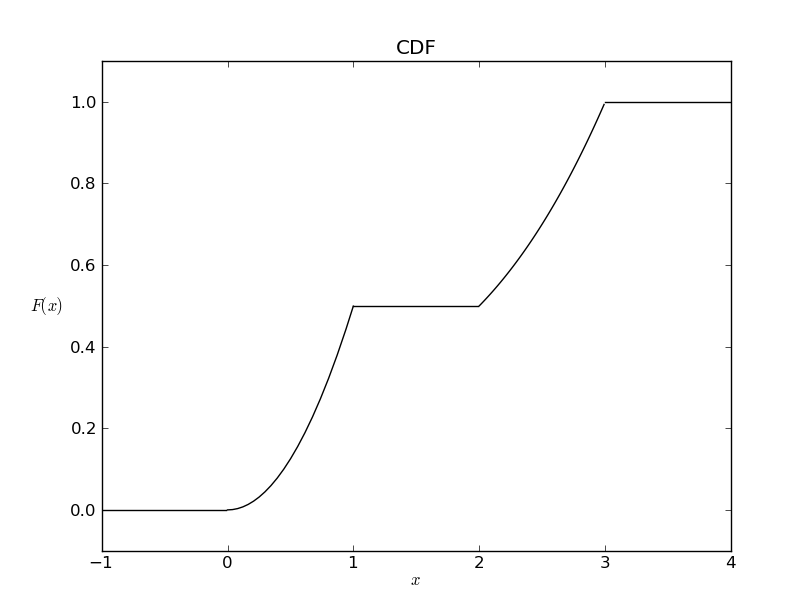
\includegraphics[scale=0.50]{problem1.png}

As can be seen from the plot, $F(x)$ is continuous everywhere. $F(x)$ is split
piecewise at the 4 points $x=0$, $x=1$, $x=2$, $x=3$. It is only
differentiable at $x=0$, where the derivative approaches 0 from both the
right and left side. It is not differentiable at the other 3 points.

\[
P(-1.5 < X < 1.8) \hspace{4px} = \hspace{4px} F(1.8) - F(-1.5) \hspace{4px}
= \hspace{4pt} \frac{1}{2} - 0 \hspace{4pt} = \hspace{4pt} \frac{1}{2}
\]

We have that $m$ is the median of $X$ iff $P(x \le m) = 1/2$ and 
$P(x \ge m) = 1/2$. These equalities hold for values of x where $F(x) = 1/2$,
which is in the interval [1,2].

\section{}

It is given by symmetry that for every possible $f(x)$, $x > a$,
there is one and only
one $f(2a-x)$, $(2a-x) < a$ such that $f(x) = f(2a-x)$. This means that:

\[
\int_{-\infty}^a f(x) dx = \int_a^{\infty} f(x) dx
\]

Since each value of df of the integral on the left side of the equation has a
corresponding and equal value of df in the integral on the right, and vice
versa. Now since the intervals of these integrals partition the real numbers
about $a$, and since $\int_{-\infty}^{\infty} f(x) dx = 1$, we have:

\[
\int_{-\infty}^a f(x) dx = \int_a^{\infty} f(x) dx = 1/2
\]

So $a$ satisfies the definition of median given at the end of Problem 1.

\section{}
Yes, each can be evaluated uniquely.

Since Gaussian distributions are symmetric about their median, the mean and
median are equal. Therefore, $\mu = 50$.

Standardizing gives:

\[
1 - 0.025 = \Phi \left( \frac{x - \mu}{\sigma} \right)
\]

\[
0.975 = \Phi \left( \frac{100 - 50}{\sigma} \right)
\]

\[
1.96 = \frac{100-50}{\sigma}
\]

\[
\sigma = \frac{100-50}{1.96} \approx 25.51
\]

\section{}
Since $|X|$ cannot take on negative values, $F(x)_{|X|}$ and $f(x)_{|X|}$ will
equal 0 for any $x < 0$. For $x \ge 0$, $f(x)_{|X|}$ will be the sum of $f(x)$
and $f(-x)$. $F(x)_{|X|}$ will include not only the area under $f(x)$ from
0 to $x$, but also the area under $f(x)$ from $-x$ to 0. So:

\[
f(x)_{|X|} = \left\{
\begin{array}{l l}
0 & x < 0\\
f(x) + f(-x) & x \ge 0\\
\end{array} \right.
\]

\[
F(x)_{|X|} = \left\{
\begin{array}{l l}
0 & x < 0\\
\int_{-x}^{x} f(x) dx & x \ge 0\\
\end{array} \right.
\]

\section{}
Standardizing gives:

\[
1 - 0.015 = \Phi \left( \frac{x-\mu}{\sigma} \right)
\]

\[
0.985 = \Phi \left( \frac{8-\mu}{0.25} \right)
\]

\[
2.17 = \frac{8-\mu}{0.25}
\]

\[
\mu = 8-(2.17)(0.25) \approx 7.46
\]

\section{}
Since we can think of the mean of a random variable as the average of all
possible values it could take, weighted by the probability of their occurence,
we have:

\[
\bar{x} = \int_{-\infty}^{\infty} xf(x)
\]

Where $f(x)$ is the p.d.f. of the continuous random variable $X$.

\begin{enumerate}[(a)]
\item
\[
\bar{x} = \int_{-\infty}^{\infty} xf(x) dx = \int_0^1 ax^a dx =
\frac{ax^{a+1}}{a+1}
\bigg{|}^{x=1} - \hspace{4pt}
\frac{ax^{a+1}}{a+1} \bigg{|}^{x=0} = \frac{a}{a+1} \hspace{4pt}-\hspace{4pt}0 =
\frac{a}{a+1}
\]

\item
\[
\bar{x} = \int_{-\infty}^{\infty} xf(x) dx = \int_0^2 x(3/2)(x-1)^2 dx = 
\int_0^2 \left( \frac{3x^3}{2} - 3x^2 + \frac{3x}{2} \right) dx =
\]

\[
\frac{3x^4}{8} - x^3 + \frac{3x^2}{4} \bigg{|}^{x=2} - 
\frac{3x^4}{8} - x^3 + \frac{3x^2}{4} \bigg{|}^{x=0} = (6 - 8 + 3) - 0 = 0
\]

\end{enumerate}
\section{}
$F(x) = 1$ for arbitrarily large values of $x$. So for arbitrarily large $x$
the area under $F(x)$ over the interval $(x,x+k) = 1k = k$. Similarly,
as $x$ goes to
infinity the area under $F(x)$ over the interval $(x+a, x+b)$ is simply
$1(b-a) = b-a$. This can be restated as:

\[
\int_{-\infty}^{\infty}[F(x+b) - F(x+a)]dx = b - a
\]

\end{document}
